\documentclass[twocolumn,superscriptaddress,aps,floatfix, nofootinbib]{revtex4-1}


%%%%%%%%%%%%
% Packages %
%%%%%%%%%%%%

\usepackage[utf8]{inputenc}

\usepackage{amsfonts}
\usepackage{amssymb}
\usepackage{amsmath}
\usepackage{amsthm}

\usepackage{bbold}
\usepackage{bm}
\usepackage{graphicx}
\usepackage{color}
\usepackage{hyperref}

\usepackage{subcaption}
\usepackage{float}


%%%%%%%%%%%%
% Document %
%%%%%%%%%%%%

\begin{document}
    % ----- Title ----- %
    
    \title{\Large{INFO8010 : Neural style transfer}}
    \vspace{1cm}
    
    \author{\small{\bf Maxime Meurisse}}
    \affiliation{\texttt{m.meurisse@student.uliege.be} (\texttt{s161278})}
    
    \author{\small{\bf Adrien Schoffeniels}}
    \affiliation{\texttt{adrien.schoffeniels@student.uliege.be} (\texttt{s162843})}
    
    \author{\small{\bf Valentin Vermeylen}}
    \affiliation{\texttt{valentin.vermeylen@student.uliege.be} (\texttt{s162864})}
    
    \maketitle
    
    %%%%%%%%%%%%%%%%%%%%
    %%%%%%%%%%%%%%%%%%%%
    %%%%%%%%%%%%%%%%%%%%
    
    % ----- Introduction ----- %
    
    % TO DO
    % -----
    % States the problem which has been tackled
    
    \section{Introduction}
    
    We decided to tackle the subject of \emph{neural style transfer} for this deep learning project. The basic idea of this subject is to \emph{merge the style of one image and the content of another image}, for example applying the style of an oil painting to a photo of an animal (Figure \ref{fig:introduction.example}).
    
    \begin{figure}[ht]
        \centering
        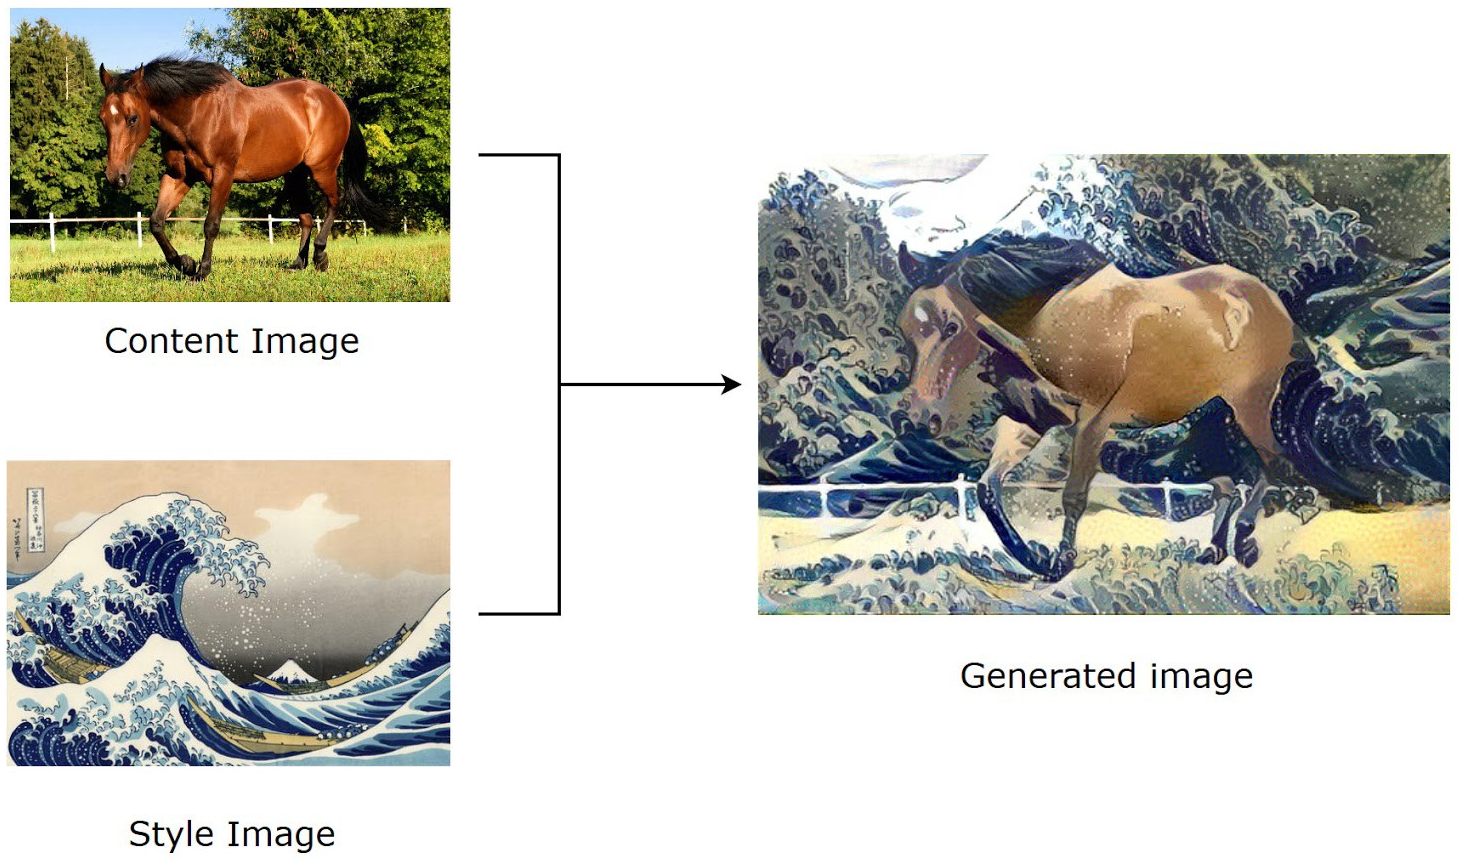
\includegraphics[width=0.45\textwidth]{resources/png/example.png}
        \caption{An example of neural style transfer (Gatys et al. technique) \cite{towardsdatascience.com}.}
        \label{fig:introduction.example}
    \end{figure}
    
    However, the rich domain of neural style transfer does not stop there, many other possible applications and extensions exist : modifying the style of a painting to make it look like a photo (and vice versa), modifying the style of certain elements of a photo (for example, transforming horses into zebras by applying a striped texture to them), transforming a summer landscape into a winter landscape, coloring an image, etc.\\
    
    The applications are many and varied. We have chosen to focus on the application of merging the style of an image and the content of another image.\\
    
    To do this, we first started by exploring the technique explained in the paper by Gatys et al. \cite{DBLP:journals/corr/GatysEB15a}. We tried to re-implement this technique ourselves, to improve it, and to vary the different parameters to understand how it works. This method is described in section \ref{sec:methods.gatys} and its results are discussed in section \ref{sec:results.gatys}.\\
    
    Secondly, we have looked at the CycleGAN (\emph{Cycle-Consistent Generative Adversarial Networks}) technique introduced in the paper by Zhu et al. \cite{DBLP:journals/corr/ZhuPIE17}. This technique, using generative adversarial networks, is very rich and allows many possible applications.\\
    
    An example of style transfer using CycleGAN is shown in Figure \ref{fig:introduction.example.cyclegan}.
    
    \begin{figure}[ht]
        \centering
        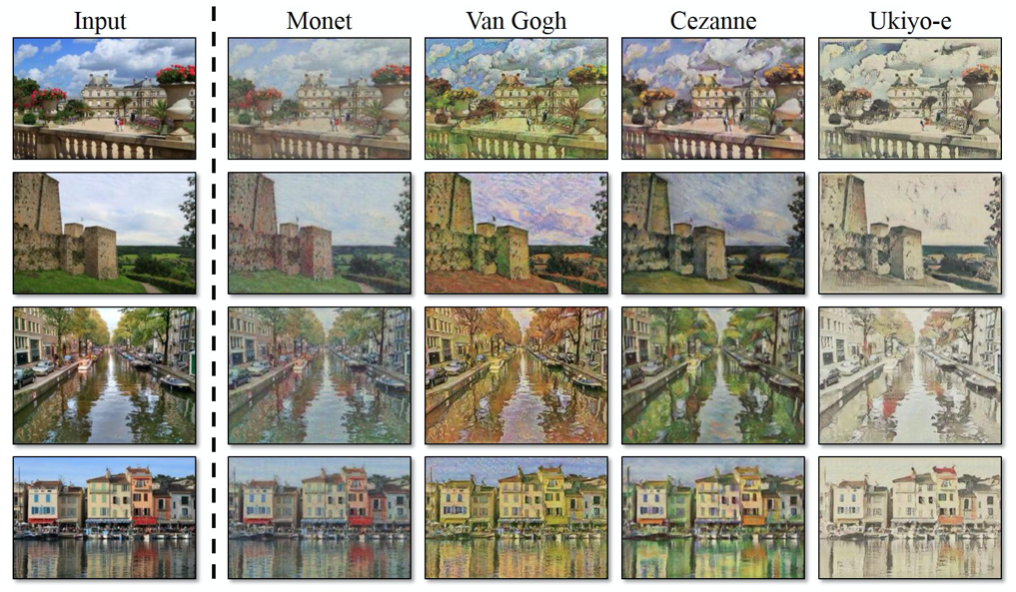
\includegraphics[width=0.45\textwidth]{resources/png/cyclegan-example.png}
        \caption{An example of neural style transfer (Zhu et al. technique) \cite{junyanz.github.io}.}
        \label{fig:introduction.example.cyclegan}
    \end{figure}
    
    We have also tried to re-implement it by ourselves and to vary its different elements. This method is described in section \ref{sec:methods.zhu} and its results are discussed in section \ref{sec:results.zhu}.\\
    
    Finally, we tried some extensions in order to dig deeper into the subject : use of different models, techniques to try to control colour (although it proved to not yield good results), etc. These results are discussed in the corresponding sections of each method. The different difficulties encountered as well as our impressions of this work and our conclusion are explained in section \ref{sec:discussion}.\\
    
    Although this report is longer than what was expected, our task relied a lot on experiments and discussion of results, and we implemented two architectures and have a lot of pictures, so we felt that restraining ourselves to 8 pages would have meant leaving a lot of our work untalked about, since we also had to explain thoroughly our methods. We are however sorry for this lengthy report.
    
    %%%%%%%%%%%%%%%%%%%%
    %%%%%%%%%%%%%%%%%%%%
    %%%%%%%%%%%%%%%%%%%%
    
    % ----- Related work ----- %
    
    % TO DO
    % -----
    % Research that is related to the considered problem
    
    \section{Related work}
    
    The field of neural style transfer and its applications are very rich. We have researched the literature to find out what the basic principles are, what the different techniques are and how they can be improved.\\
    
    We first based ourselves, as explained in the introduction, on the paper by Gatys et al. and on the paper by Zhu et al. :
    
    \begin{itemize}
        \item \cite{DBLP:journals/corr/GatysEB15a} - Paper by Gatys et al. : a paper that introduces a technique for neural style transfer using a network, such as VGG19, already trained.
        \item \cite{DBLP:journals/corr/ZhuPIE17} - Paper by Zhu et al. : a paper that introduces a technique, called CycleGAN, to perform unpaired image-to-image translation.
    \end{itemize}
    
    We then looked for some papers that could help us better understand the subject and improve our techniques. The field of style transfer in deep learning is very rich and its literature very varied. We consulted a wide range of sources but we focused on papers that were most relevant to our implemented techniques.
    
    \begin{itemize}
        \item \cite{DBLP:journals/corr/JingYFYS17} - Paper by Jing et al. :  a paper that provides a comprehensive overview of the current progress towards neural style transfer.
        \item \cite{DBLP:journals/corr/GatysEBHS16} - Paper by Gatys et al. : a paper that follows their original one (\cite{DBLP:journals/corr/GatysEB15a}) and introduces several improvements concerning the results that can be obtained. Examples are the possibility to include bitmaps, to control the colour transfer and the scale.
        \item \cite{DBLP:journals/corr/JohnsonAL16} - Paper by Johnson et al. : a paper that takes advantage of \emph{perceptual loss functions} to design a style transfer algorithm. The latter is compared with the original technique of Gatys et al.
        \item \cite{DBLP:journals/corr/LedigTHCATTWS16} - Paper by Ledig et al. : a paper that presents SRGAN, a generative adversarial network (GAN) for image super-resolution (SR). We used it for the discriminator architectures.
    \end{itemize}
    
    %%%%%%%%%%%%%%%%%%%%
    %%%%%%%%%%%%%%%%%%%%
    %%%%%%%%%%%%%%%%%%%%
    
    % ----- Methods ----- %
    
    % TO DO
    % -----
    % A clear and detailed description of the neural networks (architecture, training-parameters, loss function, data)
    
    \section{Methods}
    
    Basic deep learning notions are explained in the appendix.
    
    \subsection{Neural style transfer (Gatys et al.)}\label{sec:methods.gatys}
    
    The method presented in this section is that of the original paper that introduced neural style transfer. Although style transfer previously existed in a field called \emph{non-photorealistic rendering} and were implemented through \emph{artistic rendering} algorithms \cite{DBLP:journals/corr/JingYFYS17}, they made no use of neural networks for the task and achieved limited performance and results.\\
    
    The paper \cite{DBLP:journals/corr/GatysEB15a} makes use of convolutional neural networks to tackle the task. Those networks are the most powerful when dealing with images since they are able to quickly and efficiently detect local and global correlations in an image. Thanks to filters implemented at each layer, features of the image can be gradually extracted in a feedforward manner. The outputs of each layer consist therefore in \emph{feature maps}, which are filtered versions of the input image.\\
    
    The authors decided to use networks that were pre-trained on object recognition tasks. Such a network creates a representation of the input image that makes the object information increasingly explicit during the treatment, and the content of the image is thus given more weight than the fine details. Higher-level layers contain high-level content while lower-level ones (the first layers of the network) contain low-level details. The authors therefore used a middle-level layer for content representation, since it was closer to the content image while not having all details. On the other hand, the style is captured through correlations between the filter responses of different layers.\\
    
    The realization that made neural style transfer possible for the authors is that the style and content of an image are \emph{separable in a convolutional neural network}.\\
    
    As for the practical method proposed by the paper, they used the pre-trained VGG19 network, consisting of 16 convolutional layers and 5 pooling ones. The responses in a layer $l$ being the features maps of that layer, they can be stored in a matrix $F^l \in \mathcal{R}^{N_l\times M_l}$, where $F_{ij}^l$ is the activation of the $i^{th}$ filter at position $j$ in layer $l$, $N_l$ is the number of distinct filters at layer $l$ and $M_l$ is the size of the feature map (height times width).\\ 
    
    The loss that the authors have used in their work is the following one :
    \begin{equation}\label{eq:gatys.loss}
        \mathcal{L}_{total}(\vec{p},\vec{a},\vec{x}) = \alpha \mathcal{L}_{content}(\vec{p},\vec{x}) + \beta \mathcal{L}_{style}(\vec{a},\vec{x})
    \end{equation}
    where
    \begin{equation}
        \mathcal{L}_{\text {content}}(\vec{p}, \vec{x}, l)=\frac{1}{2} \sum_{i, j}\left(F_{i j}^{l}-P_{i j}^{l}\right)^{2}
    \end{equation}
    and
    \begin{align}
        \mathcal{L}_{\text {style}}(\vec{a}, \vec{x}) &= \sum_{l=0}^{L} w_{l} E_{l}\nonumber\\
        &= \sum_{l=0}^{L} w_{l} \frac{1}{4 N_{l}^{2} M_{l}^{2}} \sum_{i, j}\left(G_{i j}^{l}-A_{i j}^{l}\right)^{2}
    \end{align}
    The parameter $p$ is the photograph (content image), $x$ is the constructed one and $a$ is the artwork (style image). Parameters $\alpha$ and $\beta$ are simply weighting factors controlling the tradeoff between style and content. The content loss is the mean square error between the response matrix of the content image and that of the constructed image, while the style loss is defined as the weighted sum of the mean square errors between the Gram matrices for the generated image and the style one, taken over all layers considered for the style. The \emph{Gram matrix} is a mathematical element that computes the correlation between the different filter responses for a given layer.
    
    \subsubsection{Network architecture}
    
    The authors used model VGG19 as a basis : VGG19 is a convolutional neural network which consists of 16 convolutional layers (to transform images to feature maps), 5 pooling layers (to reduce the dimensions of the data) and 3 fully connected ones (at the end where every neuron in one layer are connected to every neuron in another layer) where 19 layers are trainable (convolutional and fully connected layers). This model is used to classify images.\\
    
    The authors have modified this network by inserting layers to reconstruct the image. For the content, a layer was inserted after a convolutional layer. For the style, several layers have been added after convolutional layers (as explained previously, the style is rebuilt by calculating the correlation between the different features of different layers).\\
    
    The insertion of additional layers can be done in several different places. We have chosen this architecture as a starting point : \texttt{normalization}, \texttt{conv\_1}, \texttt{style\_loss\_1}, \texttt{relu\_1}, \texttt{conv\_2}, \texttt{style\_loss\_2}, \texttt{relu\_2}, \texttt{pool\_2}, \texttt{conv\_3}, \texttt{style\_loss\_3}, \texttt{relu\_3}, \texttt{conv\_4}, \texttt{content\_loss}, \texttt{style\_loss\_4}, \texttt{relu\_4}, \texttt{pool\_4}, \texttt{conv\_5}, \texttt{style\_loss\_5}. One can notice that the architecture is not complete. Indeed, all layers after the last style layer inserted have been put aside : they are no longer useful once the content and style have been reconstructed. This first \texttt{normalization} layer is used to normalize input images in order to fit VGG19.
    
    \subsubsection{Implementation}
    
    We tried to implement this technique by ourselves with PyTorch. In order to correct our errors and improve our implementation, we used the \cite{pytorch.org} and \cite{nextjournal.com} tutorials. Our basic implementation is as faithful as possible to the paper \cite{DBLP:journals/corr/GatysEB15a} : we have taken VGG19 and inserted the new layers at the same places, we have taken the same values of the $\alpha$ and $\beta$ parameters, etc. We varied all these parameters afterwards. We didn't need to build up a large dataset of images (since we do not need to train VGG19, the output being constructed iteratively based on the style and content images); we simply downloaded images of style and content from the Internet.
    
    \subsection{CycleGAN (Zhu et al.)}\label{sec:methods.zhu}
    
    CycleGAN is a neural network that allows to perform \emph{unpaired image-to-image translation}. As described on the paper's official web page, "\emph{image-to-image translation is a class of vision and graphics problems where the goal is to learn the mapping between an input image and an output image using a training set of aligned image pairs.}" \cite{junyanz.github.io}. However, in many cases, paired images are not available. This technique has therefore been designed to support unpaired images.\\
    
    Paired images are images with a common context and common elements (for example, an image of horse in a field and an image of a zebra in the same position in more or less an identical field) while unpaired images are images that are not really the same (for example, an image of a horse in a field and an image of a zebra, not in the same position, not in the same size and not in a field).\\
    
    CycleGAN uses \emph{generative adversarial networks}.
    
    \subsubsection{Generative models}
    
    \emph{Generative models} are models capable of learning how to create data similar to the data they are provided with (training data). Intuitively, a model acting on data (e.g. writing good scientific articles) must have a good internal representation of this data. This internal representation could then be exploited to perform other tasks (e.g. classifying scientific articles).\\
    
    More practically, a generative model is a model that attempts to learn the joint probability distribution $P(x,y)$ between data $x$ and their label $y$ (where a non-generative model learns the conditional probability $P(y|x)$). Thus, the model would be able to generate a new sample $(x,y)$.
    
    \subsubsection{Generative adversarial networks}
    
    \emph{Generative adversarial networks} are models whose main idea is to put in competition two neural network models. One is called the \emph{generator} and is in charge of generating noisy data. The other is called the \emph{discriminator} and receives the training data and the noisy data from the generator and has to be able to distinguish between the two sources.\\
    
    An illustration of the structure of a generative adversarial networks is presented in Figure \ref{fig:methods.cyclegan.gan}.
    
    \begin{figure}[ht]
        \centering
        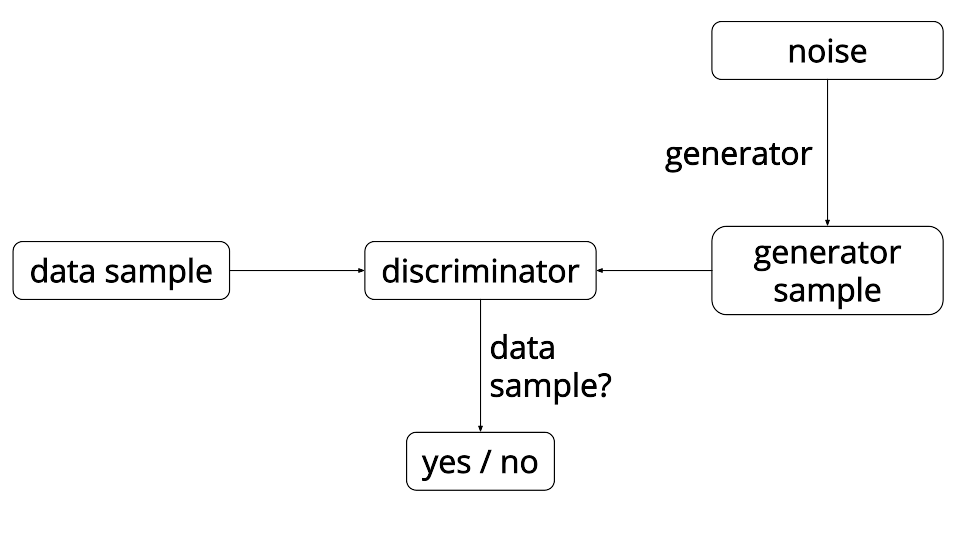
\includegraphics[width=0.45\textwidth]{resources/png/gan.png}
        \caption{Generative adversarial networks structure \cite{blog.aylien.com}.}
        \label{fig:methods.cyclegan.gan}
    \end{figure}
    
    As the training progresses, the generator produces less and less noisy data and the discriminator becomes better at distinguishing the source from the data it receives. The ultimate goal is to make the generator generate data that will be indistinguishable from the training data by the discriminator.\\
    
    In such a model, we can backpropagate gradient information from the discriminator back to the generator network, so the generator knows how to adapt its parameters in order to produce output data that can fool the discriminator. It can however be easily understood that the two networks have opposite goals, and their joint training can thus be tricky.
    
    \subsubsection{CycleGAN}
    
    Coming back to the application of neural style transfer, the idea behind the use of generative adversarial networks is \emph{to learn a mapping between the input image and the output image}. However, this technique works for paired images. CycleGAN is a technique that works on unpaired images (or more generally, unpaired input data).\\
    
    The operating principle of CycleGAN is as follows : let one set of images (for example, images of horses) in an $X$ domain and another different set of images (for example, images of zebras) in a $Y$ domain. The goal is to obtain, via training, a mapping $G : X \rightarrow Y$ and a mapping $F : Y \rightarrow X$. Mathematically, $G$ and $F$ should be inverse to each other and both mapping should be bijections. This hypothesis being made, $G$ and $F$ are trained simultaneously via a \emph{cycle consistency loss} that encourages $F(G(x)) = x$ and $G(F(y)) = y$.\\
    
    The creators of CycleGAN have exploited the fact that a translation must be "\emph{cycle consistent}" using this technique. Concretely, this means, for example, that if a sentence is translated from English into French, the re-translation of the freshly obtained French sentence into English should give the original sentence.\\
    
    Exploiting this property avoids problems such as \emph{mode collapse} : the model could generate an image which is in the domain of $Y$, and which would therefore be validated by the discriminator, without having any link with the domain $X$ (for example, generating an image of a zebra that is always the same and does not look anything like the image of the original horse).\\
    
    In total, the model contains two loss functions : an \emph{adversarial loss function} (since it is a generative adversarial model) and a \emph{cycle consistent loss function} (to take into account the cycle consistent property).\\
    
    The adversarial loss function is defined as
    \begin{align}
        \mathcal{L}_{\mathrm{GAN}}\left(G, D_{Y}, X, Y\right)&=\mathbb{E}_{y \sim p_{\text {data }}(y)}\left[\log D_{Y}(y)\right]\nonumber\\
        &+\mathbb{E}_{x \sim p_{\text {data }}(x)}\left[\log \left(1-D_{Y}(G(x))\right]\right.
    \end{align}
    where $D_Y$ is a discriminant which aims to distinguish the images ${y}$ from the translated images ${G(x)}$. They also consider the same loss for $D_X$.\\
    
    The cycle consistent loss function is defined as
    \begin{align}
        \mathcal{L}_{\text {cyc }}(G, F) &=\mathbb{E}_{x \sim p_{\text {data }}(x)}\left[\|F(G(x))-x\|_{1}\right]\nonumber\\
        &+\mathbb{E}_{y \sim p_{\text {data }}(y)}\left[\|G(F(y))-y\|_{1}\right]
    \end{align}
    taking into account that the result must satisfy the \emph{forward cycle consistency} ($x\rightarrow G(x)\rightarrow F(G(x))\approx x$) and the \emph{backward cycle consistency} ($y\rightarrow F(y)\rightarrow G(F(y))\approx y$).\\
    
    An illustration of the cycle consistent loss is shown in Figure \ref{fig:methods.cyclegan.cycleconsistentloss}.\\
    
    \begin{figure}[ht]
        \centering
        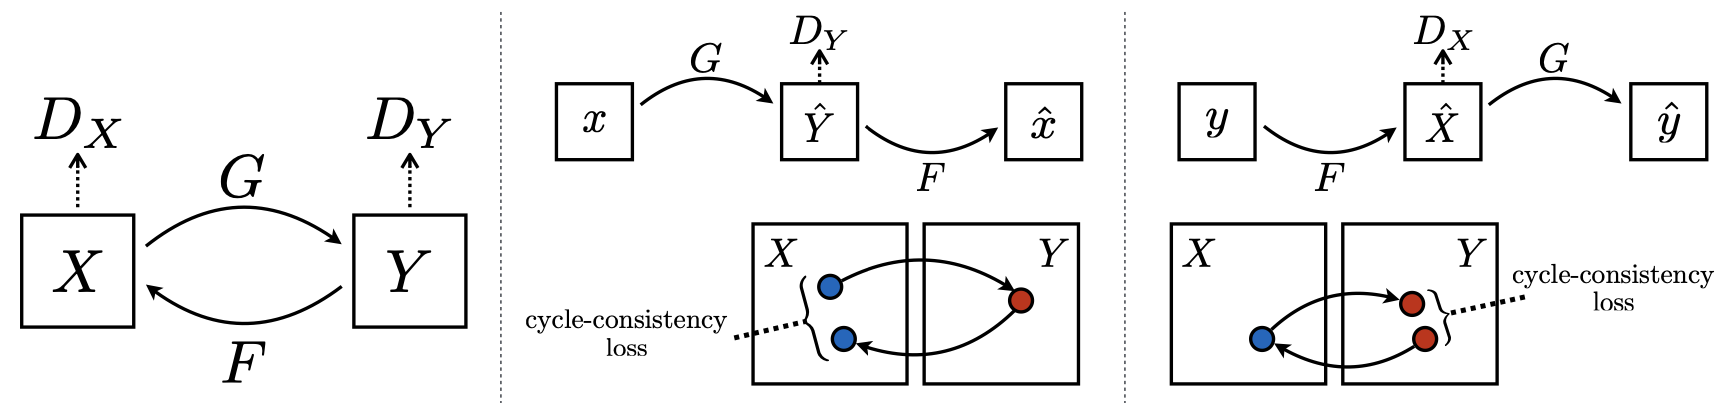
\includegraphics[width=0.45\textwidth]{resources/png/cycle-consistent-loss.png}
        \caption{Cycle consistent loss (CycleGAN) \cite{DBLP:journals/corr/ZhuPIE17}.}
        \label{fig:methods.cyclegan.cycleconsistentloss}
    \end{figure}
    
    Finally, the total (generative) loss function that the model tries to minimize is defined as
    \begin{align}
        \mathcal{L}\left(G, F, D_{X}, D_{Y}\right) &= \mathcal{L}_{\mathrm{GAN}}\left(G, D_{Y}, X, Y\right)\nonumber\\
        &+ \mathcal{L}_{\mathrm{GAN}}\left(F, D_{X}, Y, X\right)\nonumber\\
        &+ \lambda \mathcal{L}_{\mathrm{cyc}}(G, F)
    \end{align}
    where $\lambda$ controls the relative importance of the two objectives.
    
    \subsubsection{Network architectures}\label{sec:methods.cyclegan.architecture}
    
    Concerning generator architectures, the authors of CycleGAN used the architecture from Johnson et al. \cite{DBLP:journals/corr/JohnsonAL16} : 6 residual blocks for $128 \times 128$ training images and 9 residual blocks for $256 \times 256$ or higher-resolution training images.\\
    
    Concerning the discriminator architectures, they used a $70 \times 70$ PatchGAN.
    
    The exact architectures are given in the appendix.
    
    \subsubsection{Implementation}
    
    In order to implement the CycleGAN, we decided to not base ourselves upon a tutorial but instead to try to recreate the models and its training from the paper \cite{DBLP:journals/corr/ZhuPIE17} itself. We first tried to implement them from the papers it referenced before realizing that the exact architecture was given in the appendix. We thus used that source to modify the networks we implemented from their references to have the same basis as them.\\
    
    Finally, after having implemented the network, we went to the authors' GitHub repository\cite{cycgit} for the paper and compared our architecture and theirs, to make sure everything was correct. The only modification we had to make was change some reflection padding to simple padding with 0. They mentioned in their paper they used reflection padding to reduce artifacts but it was not done for all convolutional layers, so we modified that. They also used another convolutional block in their discriminator architecture, which is not mentioned in their paper.\\
    
    After the network architectures, we had to acquire a dataset of images and paintings. To do so, we used a bash script found on their GitHub repository that downloads the same datasets as they used in their research. We decided to use landscapes and Monet paintings for the two domains of interest. We also had to create a custom data loader that would return an image of both domain when called, and to do so we looked into PyTorch documentation and StackOverflow.\\
    
    For the optimizer, we reused the same one as the authors (Adam), and created a learning rate scheduler acting as they wrote in their paper (linear decrease from 1 to 0 from epoch 100 to epoch 200).\\
    
    Finally, we could start the training. The default number of epochs was set to 200, as recommended by the authors. However, we had to change the training dataset, as will be explained in the discussion section. The training first creates fake images by feeding true images to the generators, and then trains the generators by using a loss combining the cycle loss and the adversarial loss, and then trains the discriminators by comparing the output of the discriminators for the true and false images to ground truths. The sources we used for this part in order to check that what we were doing was correct were a website explaining the CycleGAN implementation in Keras\cite{keras} and a github repository of someone implementing many GANs networks\cite{erik}, as well as the authors' repository mentioned earlier. From these sources, we have taken the losses used by the authors. We have also taken inspiration for the procedure to train the network from the fourth tutorial of the course. The adversarial loss is an MSE loss, both for the generators and the discriminators, and the cycle loss and identity loss (introduced in the result section) are L1 losses.
    
    %%%%%%%%%%%%%%%%%%%%
    %%%%%%%%%%%%%%%%%%%%
    %%%%%%%%%%%%%%%%%%%%
    
    % ----- Results ----- %
    
    % TO DO
    % -----
    % Qualitative analysis : could include examples of generated images, correct vs wrong predictions, ...
    % Quantitative analysis : general overview of final performance, loss curves, comparison table with error-bars, ...
    
    \section{Results}
    
    \subsection{Neural style transfer (Gatys et al.)}\label{sec:results.gatys}
    
    In order to better understand this technique and to obtain the best results possible, we tried to vary the different parameters (and hyperparameters) controlling the model. These are listed below :
    
    \begin{itemize}
        \item input image;
        \item model used;
        \item architecture of the model used;
        \item number of steps (epochs);
        \item weights;
        \item added layers.
    \end{itemize}
    
    We discuss results obtained in a qualitative way by comparing the image obtained with the initial images and with other generated ones, and in a quantitative way by discussing the loss functions. Since this is a very visual, and therefore very subjective, application, there are few quantitative criteria to discuss. The quality of the result obtained depends very much on the user and his visual feeling. We cannot use objective quantities such as recall or accuracy, so we can only talk about the losses, and it must also be said that the general allure of the curve is more important than the actual values taken, since those depend on the weight we will give the different loss terms, and try to objectivize a subjective goal (the network does not really extract content or style, this is what we perceive, and it is not perfect in doing so). The human judgment is therefore more important than the loss for this application (the loss is useful in a given run of the network, but not so much for comparing different parameters, a task for which the human eye is better suited).
    
    \subsubsection{Input image}
    
    The input image is the image that will be generated by the model. It can be initialized in two different ways : either by taking a copy of the content image, or by taking a white noise input image. According to the literature, these two possibilities are equivalent. We have therefore tried both versions.\\
    
    We chose the \emph{Arc de Triomphe} (Paris) as the reference content image (\ref{fig:input.image.ref.content}) and some paintings as reference style images (\ref{fig:input.image.ref.style.1} and \ref{fig:input.image.ref.style.2}). These images will be used in further discussions. Obviously, the parameters that give good results for these images will not necessarily give good results for all images. We will discuss this point later.
    
    \begin{figure}[ht]
        \centering
        \begin{subfigure}[b]{0.13\textwidth}
            \centering
            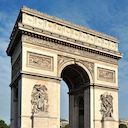
\includegraphics[width=\textwidth]{resources/png/inputs/paris.png}
            \caption{Content image}
            \label{fig:input.image.ref.content}
        \end{subfigure}
        \hfill
        \begin{subfigure}[b]{0.13\textwidth}
            \centering
            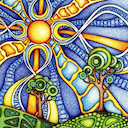
\includegraphics[width=\textwidth]{resources/png/inputs/sun-trees.png}
            \caption{Style image 1}
            \label{fig:input.image.ref.style.1}
        \end{subfigure}
        \hfill
        \begin{subfigure}[b]{0.13\textwidth}
            \centering
            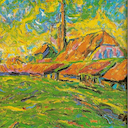
\includegraphics[width=\textwidth]{resources/png/inputs/church.png}
            \caption{Style image 2}
            \label{fig:input.image.ref.style.2}
        \end{subfigure}
        \caption{Reference images used for discussions.}
    \end{figure}
    
    For this first test, we kept the original implementation, faithful to paper \cite{DBLP:journals/corr/GatysEB15a}, with 300 epochs. The results obtained are presented in Figure \ref{fig:input.image.variations}.
    
    \begin{figure}[ht]
        \centering
        \begin{subfigure}[b]{0.22\textwidth}
            \centering
            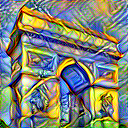
\includegraphics[width=\textwidth]{resources/png/inputs/sun-trees-paris-copy.png}
            \caption{Copy of content image}
        \end{subfigure}
        \hfill
        \begin{subfigure}[b]{0.22\textwidth}
            \centering
            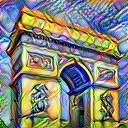
\includegraphics[width=\textwidth]{resources/png/inputs/sun-trees-paris-noisy.png}
            \caption{White noise}
        \end{subfigure}
        \caption{Starting input image.}
        \label{fig:input.image.variations}
    \end{figure}
    
    As can be seen, the results obtained are very similar. However, starting with a copy of the content image seems to give slightly smoother results for the majority of cases. For this reason, we will choose to start with a copy of the content image afterwards.
    
    \subsubsection{Model used}
    
    The authors used a pre-trained version of the VGG19 model. This version already has a set of defined weights for a better classification and therefore better results for style transfer. We tried to run the algorithm with the non pre-trained VGG19 model to compare the two versions. The results obtained are shown in Figure \ref{fig:model.pretrained.variations}.
    
    \begin{figure}[ht]
        \centering
        \begin{subfigure}[b]{0.22\textwidth}
            \centering
            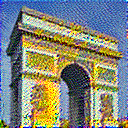
\includegraphics[width=\textwidth]{resources/png/model/sun-trees-paris-notpretrained.png}
            \caption{Not pre-trained model}
        \end{subfigure}
        \hfill
        \begin{subfigure}[b]{0.22\textwidth}
            \centering
            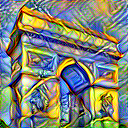
\includegraphics[width=\textwidth]{resources/png/model/sun-trees-paris-pretrained.png}
            \caption{Pre-trained model}
        \end{subfigure}
         \begin{subfigure}[b]{0.22\textwidth}
             \centering
             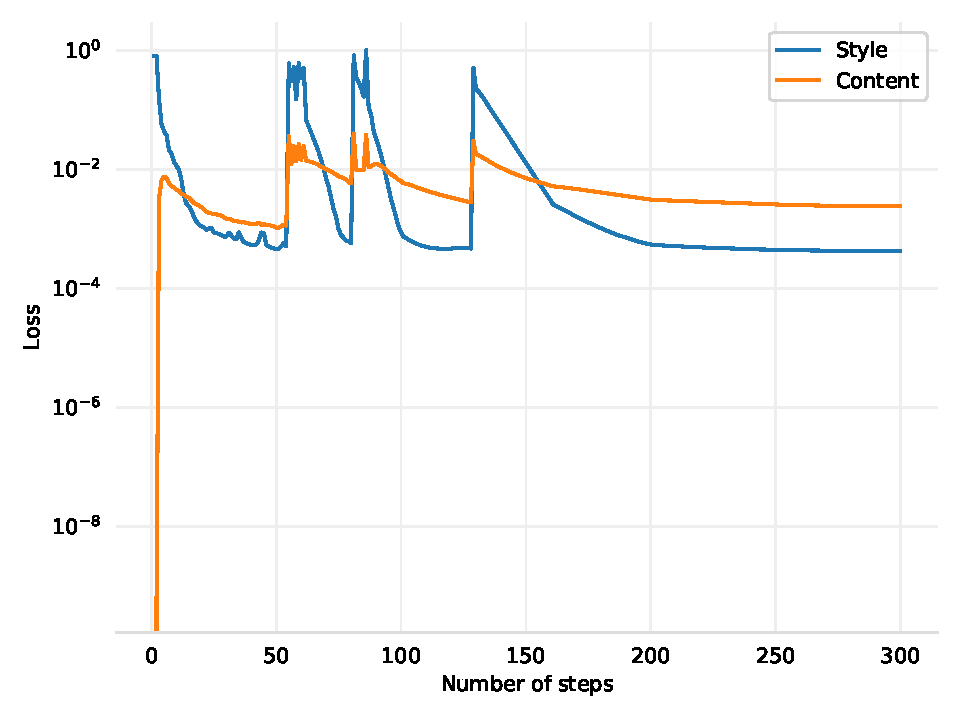
\includegraphics[width=\textwidth]{resources/pdf/model/sun-trees-paris-notpretrained.pdf}
             \caption{Not pre-trained model (loss functions)}
         \end{subfigure}
         \hfill
         \begin{subfigure}[b]{0.22\textwidth}
             \centering
             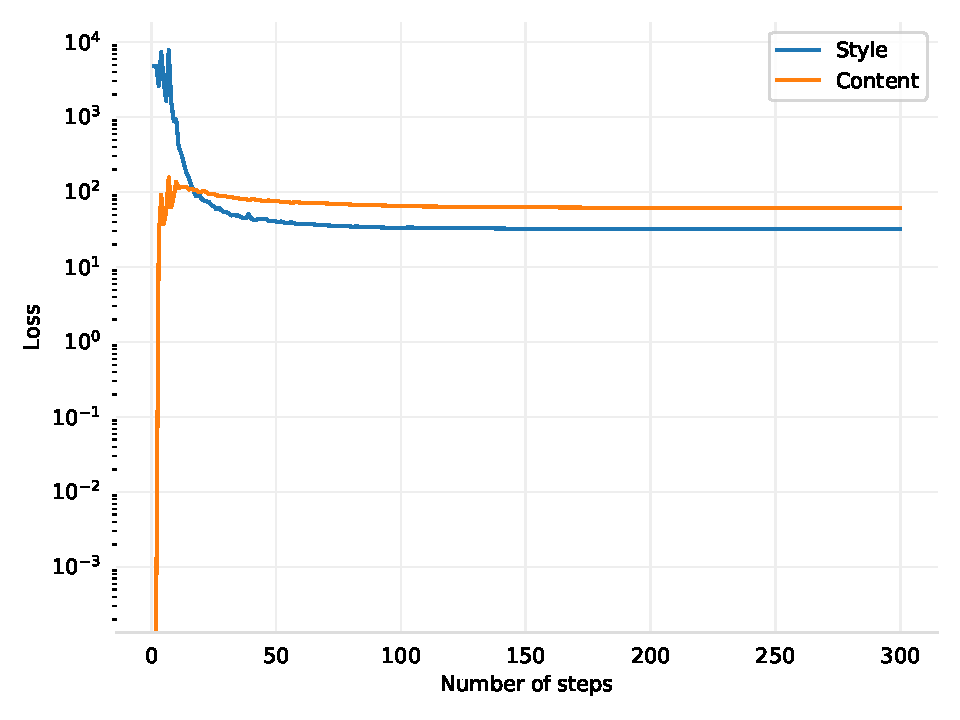
\includegraphics[width=\textwidth]{resources/pdf/model/sun-trees-paris-pretrained.pdf}
             \caption{Pre-trained model (loss functions)}
         \end{subfigure}
        \caption{VGG19 model variations.}\footnote{All loss graphs are in pdf format, so they stay clear when zooming on them.}
        \label{fig:model.pretrained.variations}
    \end{figure}
    
    We can easily observe that the pre-trained model gives much better results than the non pre-trained model. This result seems logical since the pre-trained model allows a less good extraction of the features of each image and therefore a much worse reconstruction and mix of content and style of each image. However, we can see that both networks are able to extract content (one of the first layers of the network, so the input is not yet very modified) but the not pre-trained model could not really pick up the style, which lead us to believe that networks trained on object recognition make use of the style for their task.
    
    When looking at the losses, we see that the not pre-trained model has losses that are much smaller, but that also start much smaller. Since it has not been trained on image detection first, the backpropagation makes it so that the losses are reduced, although style is not extracted (the information conveyed by layers do not have the same meaning as for the trained model). Using a different scheduler also yields poor results. The value of the loss is thus less important than our visual perception of the result.\\
    
    We tried to increase the number of epochs of the algorithm with the non pre-trained model, but the results obtained are systematically much lower than the results with the pre-trained model. To obtain better results, we should have trained the VGG19 model beforehand. Since image classification was not the main subject of our project, we worked directly with the pre-trained model afterwards.\\
    
    We also tried several other architectures to determine whether or not they may provide as good/better results than the VGG architecture. We first started with the \textbf{Alexnet} network, but the results were far from satisfactory, as can be expected from such a simple network (containing only eight layers) \cite{Krizhevsky2012ImageNetCW}.\\
    
    The next one we tried was \textbf{GoogLeNet}. However, due to its structure containing parallel blocks and bypassing links, inserting style losses inside the Inception modules while maintaining its pretrained weights proved to be very difficult. We therefore only tried to insert such layers where only one path was possible, but it lead to very poor results.\\
    
    The results of these two architectures are given at figure \ref{fig:arch.vars}.
    
    \begin{figure}[ht]
        \centering
        \begin{subfigure}[b]{0.22\textwidth}
            \centering
            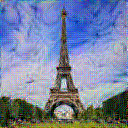
\includegraphics[width=\textwidth]{resources/png/model/googlenet.png}
            \caption{GoogLeNet architecture}
        \end{subfigure}
        \hfill
        \begin{subfigure}[b]{0.22\textwidth}
            \centering
            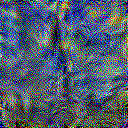
\includegraphics[width=\textwidth]{resources/png/model/alexnet.png}
            \caption{Alexnet architecture}
        \end{subfigure}
        \caption{General architecture variations.}
        \label{fig:arch.vars}
    \end{figure}
    
    \subsubsection{Architecture of the model used}
    
    The original architecture of VGG19 has max pooling layers. The authors suggest in their paper to replace these max pooling layers by average pooling layers in order to obtain more appealing results. We have therefore compared the results with these two types of layers (Figure \ref{fig:model.architecture.variations}).
    
    \begin{figure}[ht]
        \centering
        \begin{subfigure}[b]{0.22\textwidth}
            \centering
            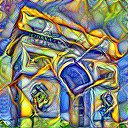
\includegraphics[width=\textwidth]{resources/png/architecture/sun-trees-paris-maxpool.png}
            \caption{Max pooling layers}
        \end{subfigure}
        \hfill
        \begin{subfigure}[b]{0.22\textwidth}
            \centering
            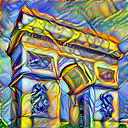
\includegraphics[width=\textwidth]{resources/png/architecture/sun-trees-paris-avgpool.png}
            \caption{Average pooling layers}
        \end{subfigure}
        \caption{VGG19 model architecture variations.}
        \label{fig:model.architecture.variations}
    \end{figure}
    
    At first glance, both results seem to be very good. However, in general, some images give very bad results with average pooling layers (while results with max pooling layers are always very good). We have therefore observed the evolution of the loss functions (Figure \ref{fig:model.architecture.loss}).
    
    \begin{figure}[ht]
        \centering
        \begin{subfigure}[b]{0.22\textwidth}
            \centering
            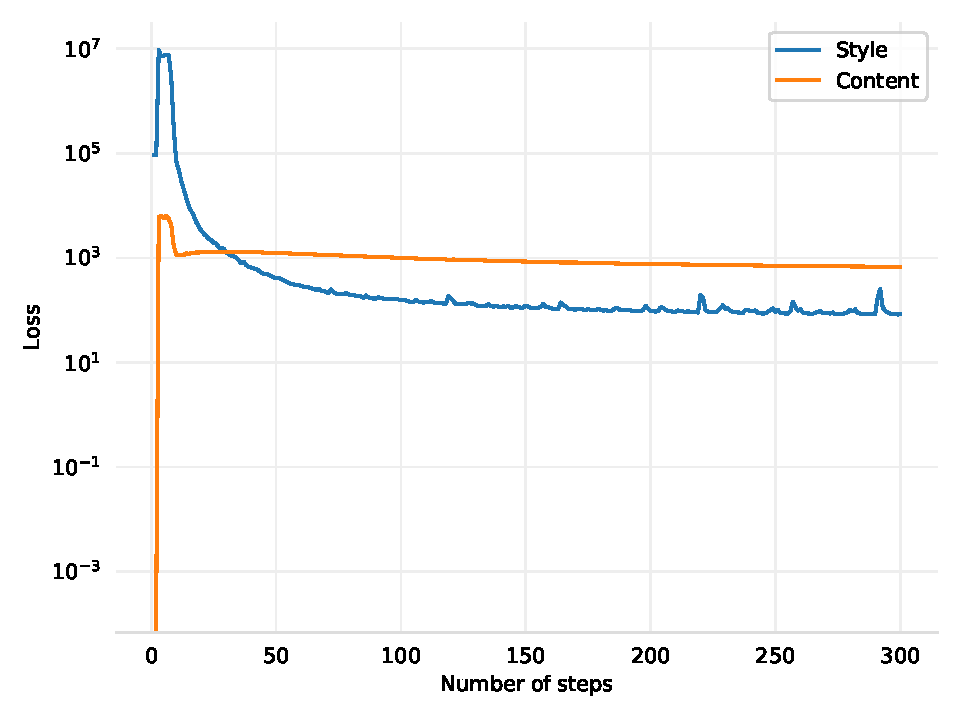
\includegraphics[width=\textwidth]{resources/pdf/architecture/sun-trees-paris-maxpool.pdf}
            \caption{Max pooling layers}
        \end{subfigure}
        \hfill
        \begin{subfigure}[b]{0.22\textwidth}
            \centering
            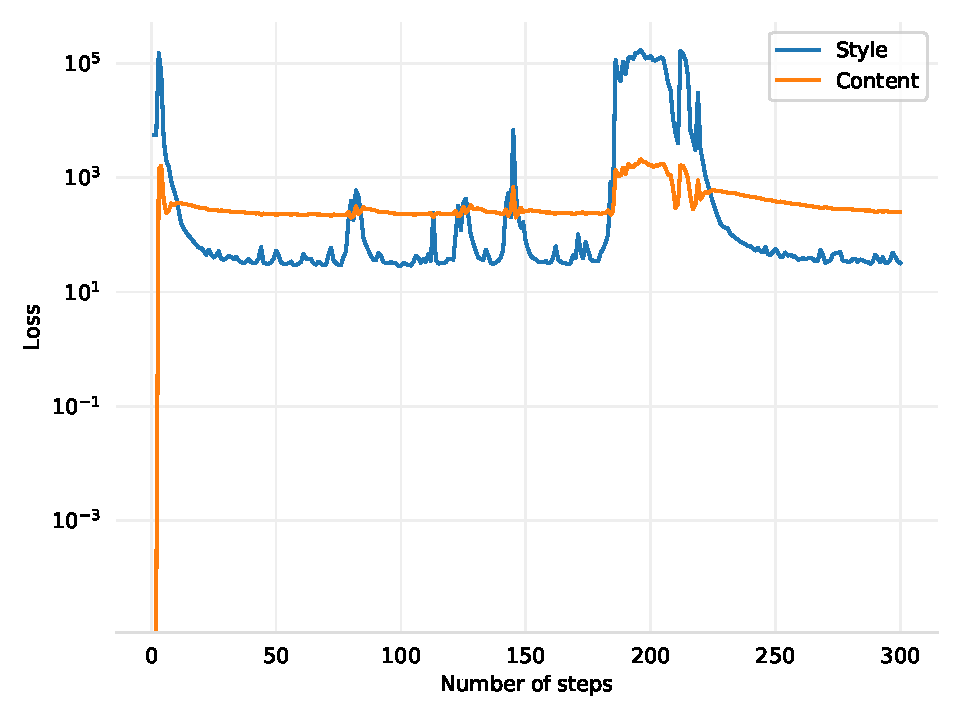
\includegraphics[width=\textwidth]{resources/pdf/architecture/sun-trees-paris-avgpool.pdf}
            \caption{Average pooling layers}
        \end{subfigure}
        \caption{VGG19 model architecture loss functions\footnote{All losses are in pdf format, to allow them to be clear while zooming.}.}
        \label{fig:model.architecture.loss}
    \end{figure}
    
    We observe that in the case of an architecture with average pooling layers, the loss functions (and especially the one concerning the content) vary strongly during the epochs while in the case of max pooling layers, the loss functions remain stable. This could explain the very bad results obtained on some images with average pooling layers.\\
    
    To overcome this, we have added a learning rate \emph{scheduler} (with a step size of 50 and a gamma multiplicator parameter of 0.3) when working with average pooling layers. This scheduler allows to reduce the learning rate as epochs pass, and thus to reduce the variations of the loss functions (the sudden high spikes were due to a too high learning rate, the model could not do anything but have its loss jump out of the potential well). We then restarted the algorithm with this scheduler (Figure \ref{fig:model.architecture.loss.scheduler}).
    
    \begin{figure}[ht]
        \centering
        \begin{subfigure}[b]{0.22\textwidth}
            \centering
            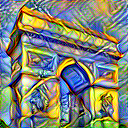
\includegraphics[width=\textwidth]{resources/png/architecture/sun-trees-paris-avgpool-scheduler.png}
            \caption{Transformed input image}
        \end{subfigure}
        \hfill
        \begin{subfigure}[b]{0.22\textwidth}
            \centering
            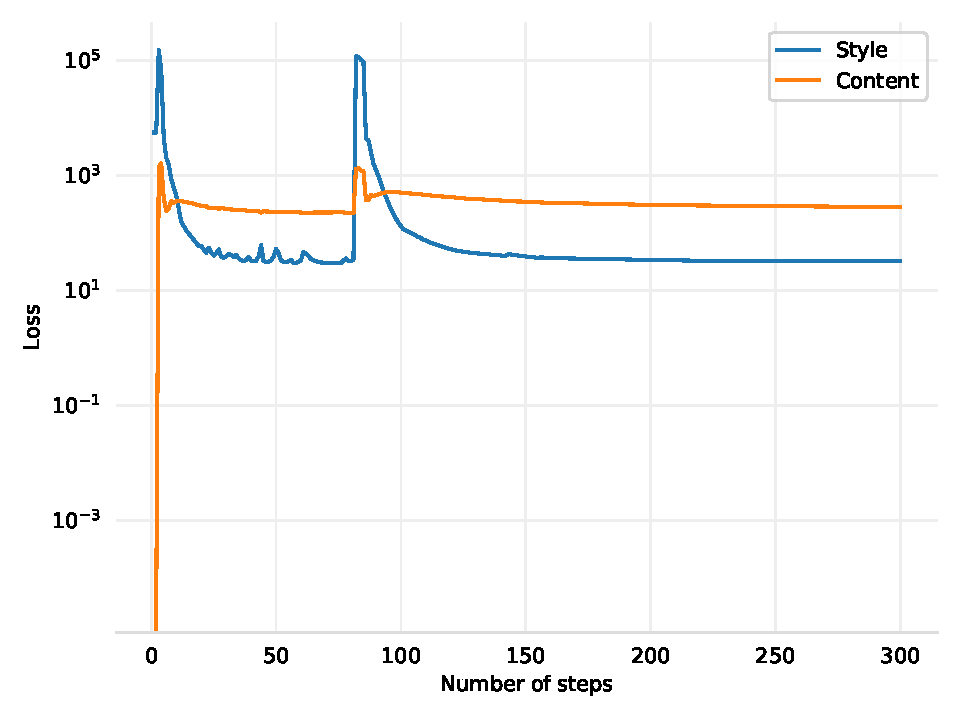
\includegraphics[width=\textwidth]{resources/pdf/architecture/sun-trees-paris-avgpool-scheduler.pdf}
            \caption{Loss functions}
        \end{subfigure}
        \caption{Average pooling layers with scheduler (VGG19).}
        \label{fig:model.architecture.loss.scheduler}
    \end{figure}
    
    We observe that the scheduler seems to be efficient since the variations of the loss functions have almost completely disappeared (a sharper decrease would remove the spike, but is dependent on the other parameters). In general, the results that were previously bad have turned out to be very good with the scheduler. The images obtained with average pooling layer seem to be smoother. So we kept this type of layer (with a scheduler).
    
    \subsubsection{Number of steps (epochs)}
    
    By default, we have set the number of steps (epochs) to 300. The results are obtained quickly and seem to be good. When we observe the loss functions (Figure \ref{fig:model.architecture.loss.scheduler} for example), we realize that they stabilize quite quickly (after about 300 epochs), whatever the scheduler we chose (since the learning rate decreases over time, the losses end up converging).
    
    In order to confirm this result, we ran the algorithm by increasing the number of epochs to 1000. The result obtained is shown in Figure \ref{fig:number.steps.variations}.
    
    \begin{figure}[ht]
        \centering
        \begin{subfigure}[b]{0.22\textwidth}
            \centering
            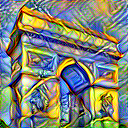
\includegraphics[width=\textwidth]{resources/png/steps/sun-trees-paris-300.png}
            \caption{300 epochs}
        \end{subfigure}
        \hfill
        \begin{subfigure}[b]{0.22\textwidth}
            \centering
            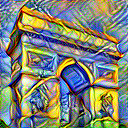
\includegraphics[width=\textwidth]{resources/png/steps/sun-trees-paris-1000.png}
            \caption{1000 epochs}
        \end{subfigure}
        \caption{Number of steps (epochs) variations.}
        \label{fig:number.steps.variations}
    \end{figure}
    
    As expected, the two results are exactly the same. Indeed, considering the evolution of the loss functions (Figure \ref{fig:number.steps.loss.functions}) per 1000 epochs, we can confirm that they stabilize quite quickly. We have therefore set the number of epochs to 300 by default.
    
    \begin{figure}[ht]
        \centering
        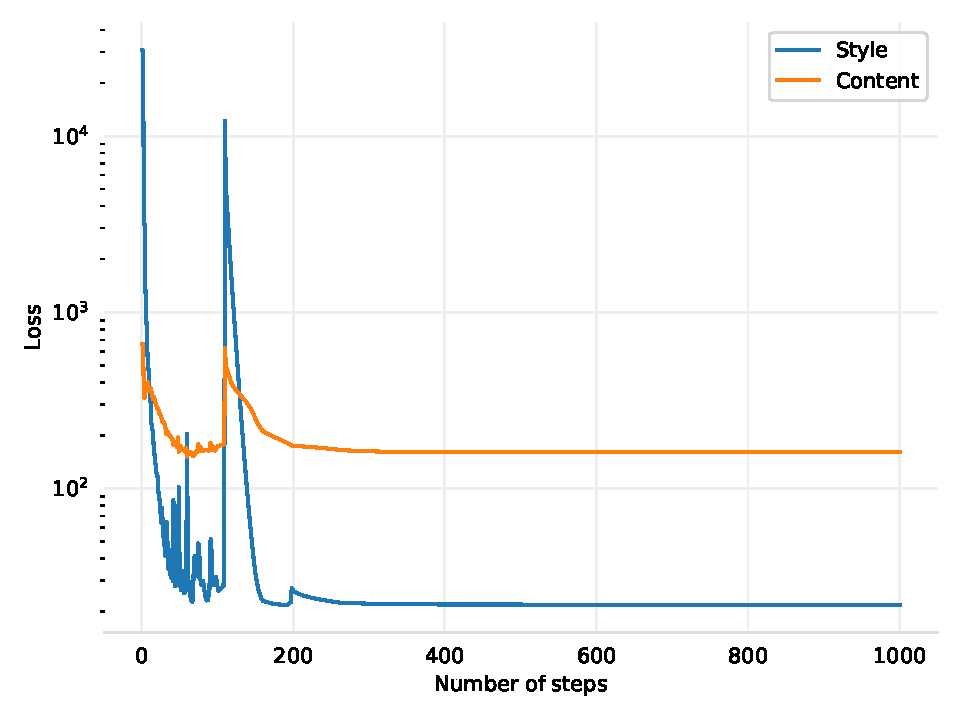
\includegraphics[width=0.45\textwidth]{resources/pdf/steps/sun-trees-paris-1000.pdf}
        \caption{Loss functions for 1000 epochs.}
        \label{fig:number.steps.loss.functions}
    \end{figure}
    
    \subsubsection{Weights}
    
    It is possible to vary the $\alpha$ and $\beta$ weights in the loss function \eqref{eq:gatys.loss}. These weights are used to distribute the style and content of the resulting image. In their paper, the authors use an $\alpha/\beta$ ratio equals to $10^{-4}$. We have tried several ratios to observe the variations of the results obtained (Figure \ref{fig:weights.ratio}).
    
    \begin{figure}[ht]
        \centering
        \begin{subfigure}[b]{0.13\textwidth}
            \centering
            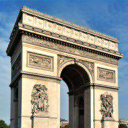
\includegraphics[width=\textwidth]{resources/png/weights/sun-trees-paris-10-2.png}
            \caption{$10^{-2}$}
        \end{subfigure}
        \hfill
        \begin{subfigure}[b]{0.13\textwidth}
            \centering
            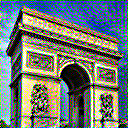
\includegraphics[width=\textwidth]{resources/png/weights/sun-trees-paris-10-3.png}
            \caption{$10^{-3}$}
        \end{subfigure}
        \hfill
        \begin{subfigure}[b]{0.13\textwidth}
            \centering
            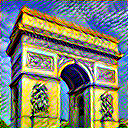
\includegraphics[width=\textwidth]{resources/png/weights/sun-trees-paris-10-4.png}
            \caption{$10^{-4}$}
        \end{subfigure}
        \begin{subfigure}[b]{0.13\textwidth}
            \centering
            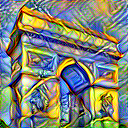
\includegraphics[width=\textwidth]{resources/png/weights/sun-trees-paris-10-5.png}
            \caption{$10^{-5}$}
        \end{subfigure}
        \hfill
        \begin{subfigure}[b]{0.13\textwidth}
            \centering
            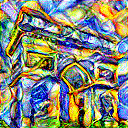
\includegraphics[width=\textwidth]{resources/png/weights/sun-trees-paris-10-6.png}
            \caption{$10^{-6}$}
        \end{subfigure}
        \hfill
        \begin{subfigure}[b]{0.13\textwidth}
            \centering
            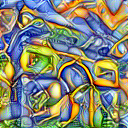
\includegraphics[width=\textwidth]{resources/png/weights/sun-trees-paris-10-7.png}
            \caption{$10^{-7}$}
        \end{subfigure}
        \caption{Results for different values of ratio $\alpha/\beta$.}
        \label{fig:weights.ratio}
    \end{figure}
    
    We observe that if the ratio is too high ($10^{-2}$), the result is not influenced at all by the style image and, on the contrary, if the ratio is too low ($10^{-7}$), the style totally takes over the result. A suitable ratio seems to be around $10^{-5}$. This result is of course highly dependent on the images and the expected result : a low contrast style image with dull colors will require a very low ratio to appear while a very bright and colorful style image will appear with a higher ratio. In general, the $10^{-5}$ ratio seems to give good results for all image combinations. We have therefore kept this value.\\
    
    We note that the $\alpha$ value is much smaller than the $\beta$ value. Indeed, the base image being a copy of the content image, it is not necessary to greatly modify it from a content point of view. Furthermore, we need a value for one of the two weights to determine the other, and the best results were obtained with a content weight of 10.\\
    
    We also tried to assign a weight to each layer added to rebuild the style image. Indeed, the authors mention in their paper that "\emph{[...] when matching the style representations up to higher layers in the network, local images structures are matched on an increasingly large scale, leading to a smoother and more continuous visual experience. Thus, the visually most appealing images are usually created by matching the style representation up to the highest layers in the network. [...]}" \cite{DBLP:journals/corr/GatysEB15a}. We therefore varied the influence of the different layers used to rebuild the style image by assigning them different weights (Figure \ref{fig:weights.style.layers}).

    \begin{figure}[ht]
        \centering
        \begin{subfigure}[b]{0.13\textwidth}
            \centering
            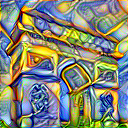
\includegraphics[width=\textwidth]{resources/png/weights/sun-trees-paris-equals-weights.png}
            \caption{$w = [1, 1, 1, 1, 1]$}
        \end{subfigure}
        \hfill
        \begin{subfigure}[b]{0.13\textwidth}
            \centering
            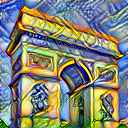
\includegraphics[width=\textwidth]{resources/png/weights/sun-trees-paris-linear-decreasing-weights.png}
            \caption{$w = [1, .8, .6, .4, .2]$}
        \end{subfigure}
        \hfill
        \begin{subfigure}[b]{0.13\textwidth}
            \centering
            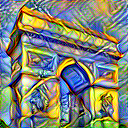
\includegraphics[width=\textwidth]{resources/png/weights/sun-trees-paris-high-decreasing-weights.png}
            \caption{$w = [.75, .5, .2, .2, .2]$}
        \end{subfigure}
        \caption{Style layers' weights variations.}
        \label{fig:weights.style.layers}
    \end{figure}
    
    We get different results, but each one is very good. We find that, logically, by assigning less weight to the different style layers (especially the last ones), we obtain results where the style is less marked. Again, the ratings are very subjective and depend on the user's desired results.
    
    \subsubsection{Added layers}
    
    The authors mention in their paper that the layers considered to reconstruct the image of content and the image of style have a significant influence on the result. The content image is rebuilt after a convolutional layer and the style image is rebuilt based on a correlation of filters of several layers. We tried to put them at different places inside the VGG19 model in order to observe the influence on the result obtained and try to find the best configuration. The results are shown in Figure \ref{fig:added.layers}. Only one style layer is used in order to best see its impact, although several are used in practice.
    
    \begin{figure}[ht]
        \centering
        \begin{subfigure}[b]{0.1\textwidth}
            \centering
            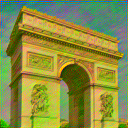
\includegraphics[width=\textwidth]{resources/png/layers/conv1_conv1.png}
            \caption{$s$: conv1  $c$: conv1}
            \label{fig:added.layers.s1.c1}
        \end{subfigure}
        \hfill
        \begin{subfigure}[b]{0.1\textwidth}
            \centering
            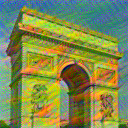
\includegraphics[width=\textwidth]{resources/png/layers/conv3_conv1.png}
            \caption{$s$: conv3 $c$: conv1}
            \label{fig:added.layers.s3.c1}
        \end{subfigure}
        \hfill
        \begin{subfigure}[b]{0.1\textwidth}
            \centering
            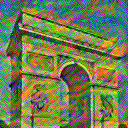
\includegraphics[width=\textwidth]{resources/png/layers/conv5_conv1.png}
            \caption{$s$: conv5 $c$: conv1}
            \label{fig:added.layers.s5.c1}
        \end{subfigure}
        \hfill
        \begin{subfigure}[b]{0.1\textwidth}
            \centering
            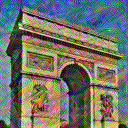
\includegraphics[width=\textwidth]{resources/png/layers/conv9_conv1.png}
            \caption{$s$: conv9 $c$: conv1}
            \label{fig:added.layers.s9.c1}
        \end{subfigure}
        \begin{subfigure}[b]{0.1\textwidth}
            \centering
            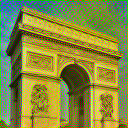
\includegraphics[width=\textwidth]{resources/png/layers/conv1_conv3.png}
            \caption{$s$: conv1 $c$: conv3}
            \label{fig:added.layers.s1.c3}
        \end{subfigure}
        \hfill
        \begin{subfigure}[b]{0.1\textwidth}
            \centering
            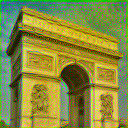
\includegraphics[width=\textwidth]{resources/png/layers/conv1_conv5.png}
            \caption{$s$: conv1 $c$: conv5}
            \label{fig:added.layers.s1.c5}
        \end{subfigure}
        \hfill
        \begin{subfigure}[b]{0.1\textwidth}
            \centering
            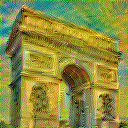
\includegraphics[width=\textwidth]{resources/png/layers/conv1_conv9.png}
            \caption{$s$: conv1 $c$: conv9}
            \label{fig:added.layers.s1.c9}
        \end{subfigure}
        \hfill
        \begin{subfigure}[b]{0.1\textwidth}
            \centering
            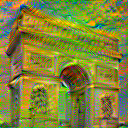
\includegraphics[width=\textwidth]{resources/png/layers/conv3_conv9.png}
            \caption{$s$: conv3 $c$: conv9}
            \label{fig:added.layers.s3.c9}
        \end{subfigure}
        \caption{Influence of the position of the construction layers ($s$ is the layer after which the style layer is positioned, $c$ is the layer after which the content layer is placed).}
        \label{fig:added.layers}
    \end{figure}
    
    As shown by the figures \ref{fig:added.layers.s1.c1}, \ref{fig:added.layers.s3.c1}, \ref{fig:added.layers.s5.c1} and \ref{fig:added.layers.s9.c1}, the style seems to be better reproduced when the style layer is placed in the beginning of the network. When it's placed after the first convolutional layer, the general color scheme is well respected but the colour shifts are smooth. We do not perceive brush strokes as they are in the original image. As we move the layer along the network, the colour scheme is less and less well-reproduced, but the structure of the style image (the brush strokes) is more and more visible. This is the result expected since the higher convolutional layers capture higher level content. In accordance with these subjective observations, we found that the style loss increases when the layer is moved along the network (see Figure \ref{fig:loss.layers.style}). Note that from the 9th layer, the loss begins to lessens, but subjectively we can see that the style isn't as well reproduced as for previous layers.\\
    
    In the same way, when we move the content layer along the network (as shown by the figures \ref{fig:added.layers.s1.c1}, \ref{fig:added.layers.s1.c3}, \ref{fig:added.layers.s1.c5} and \ref{fig:added.layers.s1.c9}), the representation of the monument becomes less and less precise, since low-level convolutional layers care about details while high-level ones care more about objects and their arrangement, without too much details. This way, placing the content layer  further in the network allows to better apply the style to the image (it does not seem to be a picture with a filter on top anymore). Once again the style loss confirms these observations as it lessens when the content layer advances in the network, except for the first layer but, subjectively, the content then looks too similar to the one of the original image, as we have just mentioned (see Figure \ref{fig:loss.layers.content}).\\

    \begin{figure}[ht]
        \centering
        \begin{subfigure}[b]{0.22\textwidth}
            \centering
            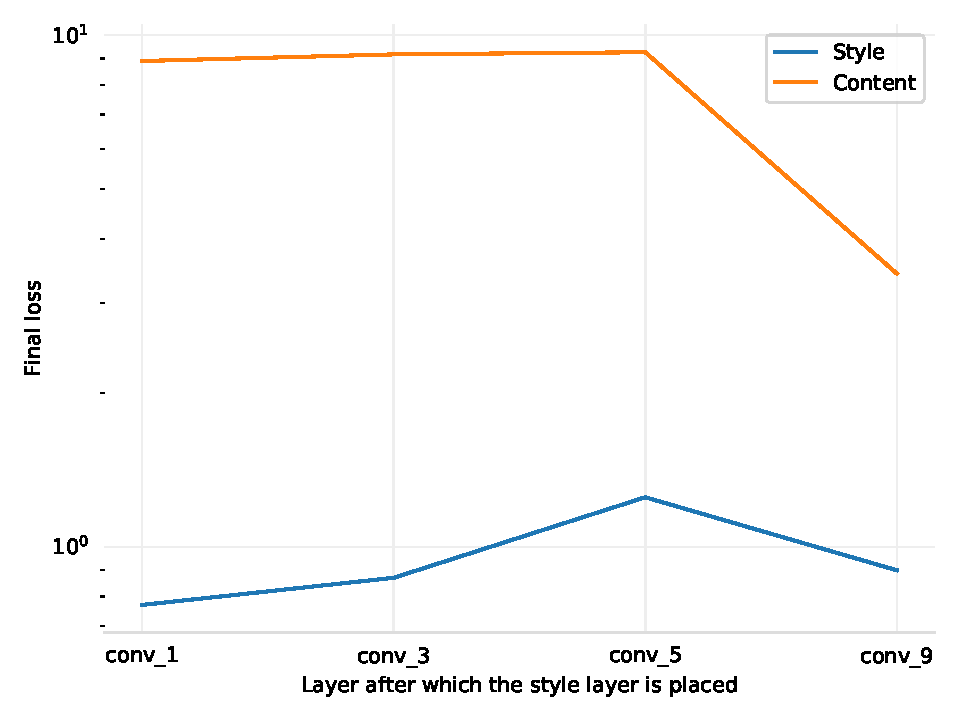
\includegraphics[width=\textwidth]{resources/png/layers/style_losses.pdf}
            \caption{Style layer}
            \label{fig:loss.layers.style}
        \end{subfigure}
        \hfill
        \begin{subfigure}[b]{0.22\textwidth}
            \centering
            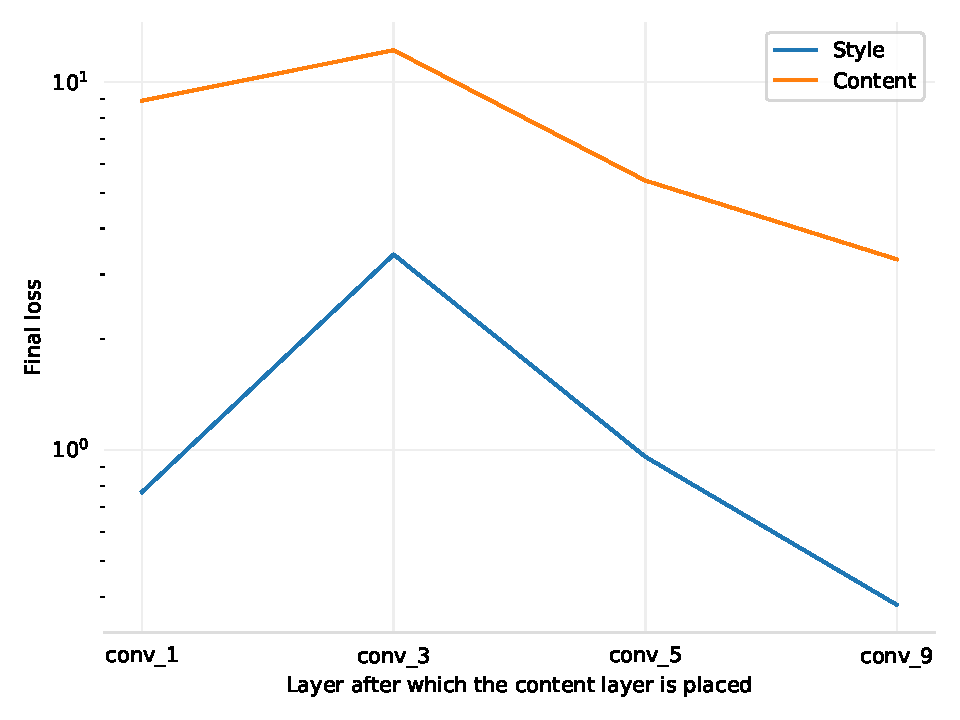
\includegraphics[width=\textwidth]{resources/png/layers/content_losses.pdf}
            \caption{Content layer}
            \label{fig:loss.layers.content}
        \end{subfigure}
        \caption{Evolution of the losses depending on the places of the style and content layers.}
        \label{fig:loss.layers}
    \end{figure}
    
    Based on these findings, we manage to get nice results by placing the style layers at different locations in the network (to get the right colours, but also a little bit of the form of the style picture), but giving more weight to the ones that come first, and by placing the content layer around the middle of the network (the exact location can be adapted according to the input images). An example of what can be achieved is shown in Figure \ref{fig:added.layer.result}. 
    
    \begin{figure}[ht]
        \centering
        \begin{subfigure}[b]{0.22\textwidth}
            \centering
            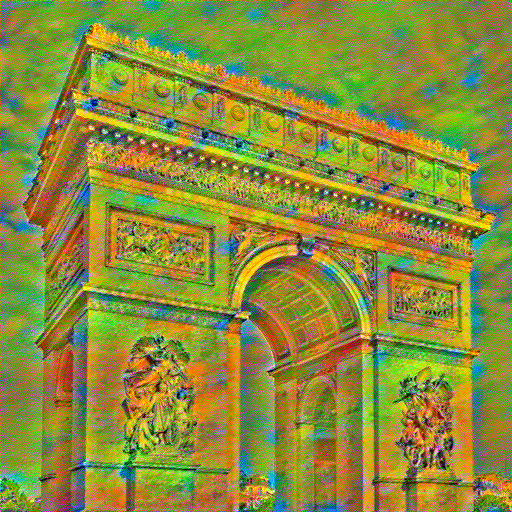
\includegraphics[width=\textwidth]{resources/png/layers/layers_default.png}
            \caption{Starting architecture}
        \end{subfigure}
        \hfill
        \begin{subfigure}[b]{0.22\textwidth}
            \centering
            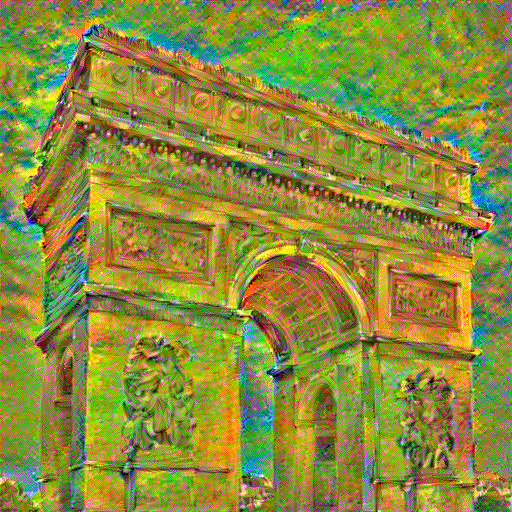
\includegraphics[width=\textwidth]{resources/png/layers/layers_nicer.png}
            \caption{Modified architecture}
            \label{fig:added.layer.result}
        \end{subfigure}
        \caption{Comparison of the result that can be achieved by modifying the network architecture with the starting point architecture.}
    \end{figure}
    
    \subsubsection{Final results}
    
    We have tried to explore the technique of Gatys et al. and to vary its different parameters in order to better understand it. In summary, we observed that taking as input image a copy of the content image gives smoother results; a pre-trained model logically gives better results; average pooling layers (with a scheduler) give, on average, better results; 300 epochs seem to be sufficient and that, finally, a ratio of $10^{-5}$ between the weight of the content (set to 10) and the weight of the style seems to be good on average. Other parameters such as where new layers are added and the weights assigned to these layers depend very strongly on the input images and the desired results.\\
    
    We applied the algorithm to a whole series of images, adjusting the parameters as best we could according to the different discussions made previously. Our results are presented in Figure \ref{fig:final.results.gatys}.
    
    \begin{figure*}
        \centering
        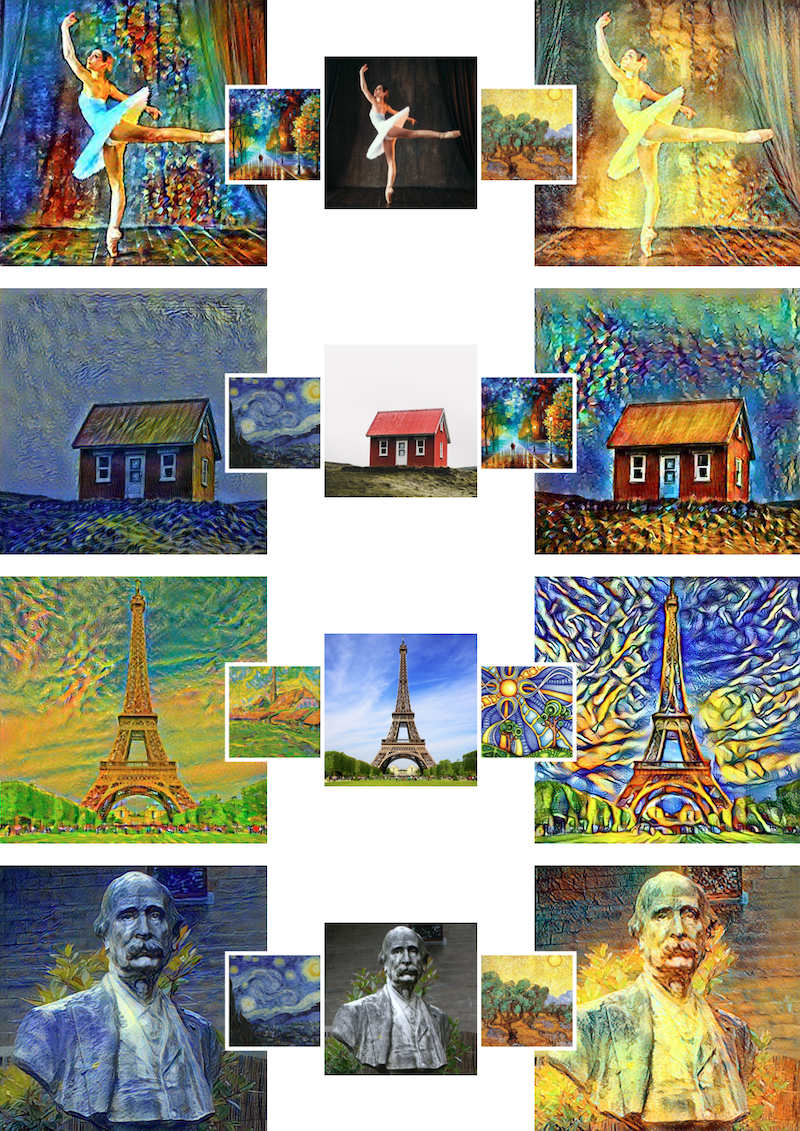
\includegraphics[width=0.90\textwidth]{resources/png/gatys-final.png}
        \caption{Some results obtained with Gatys et al. technique.}
        \label{fig:final.results.gatys}
    \end{figure*}
    
    \subsection{CycleGAN (Zhu et al.)}\label{sec:results.zhu}
    
    When implementing the paper, we decided to use the dataset "Monet and landscapes", found on the authors' github page\cite{cycgit}. However, when launching our script, we quickly realized that, with the low resources we could obtain at one time on the GPU, we would not be able to train the network on the 7000 images on the training sets. Indeed, training the model for 200 epochs (as recommended by the authors) on 20 batches of 3 images of each domain per epoch took us between 40 and 50 hours. We therefore had to test strategies to have results by the deadline for the project. These strategies and their results are discussed here, as well as - our attempts for explaining the different results. The input landscape image to be translated into Monet's style is given at Figure \ref{fig:landscape}. It can be noted that the difference of results between images used in the training or not was not visible to us.
    \begin{figure}[H]
        \centering
        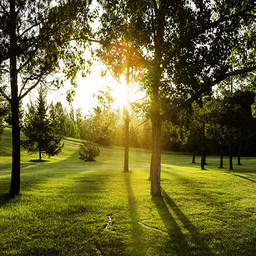
\includegraphics[scale=0.5]{resources/png/inputs/test.jpg}
        \caption{Input image for CycleGAN}
        \label{fig:landscape}
    \end{figure}
    
    \subsubsection{Limiting the number of batches per epochs}\label{limiting}
    
    This is the strategy that lead to the 40-50 hours stated above. Here, we decided to use the training set and to restrict the number of batches per epoch at 20 (containing 3 images of each style). One result as well as the losses can be seen in Figure \ref{fig:limitation}. As can be seen, the result is disappointing but can be explained by the fact that the generator has not been able to improve and reduce its loss, while the discriminator loss decreased greatly over the epochs. This may be a case of vanishing gradient. We believe it may come from the fact that the training dataset was too small. Indeed, over 200 epochs, we only passed twice through all the dataset (containing more than 6000 images).
    
    \begin{figure}[H]
        \centering
        \begin{subfigure}[b]{0.22\textwidth}
            \centering
            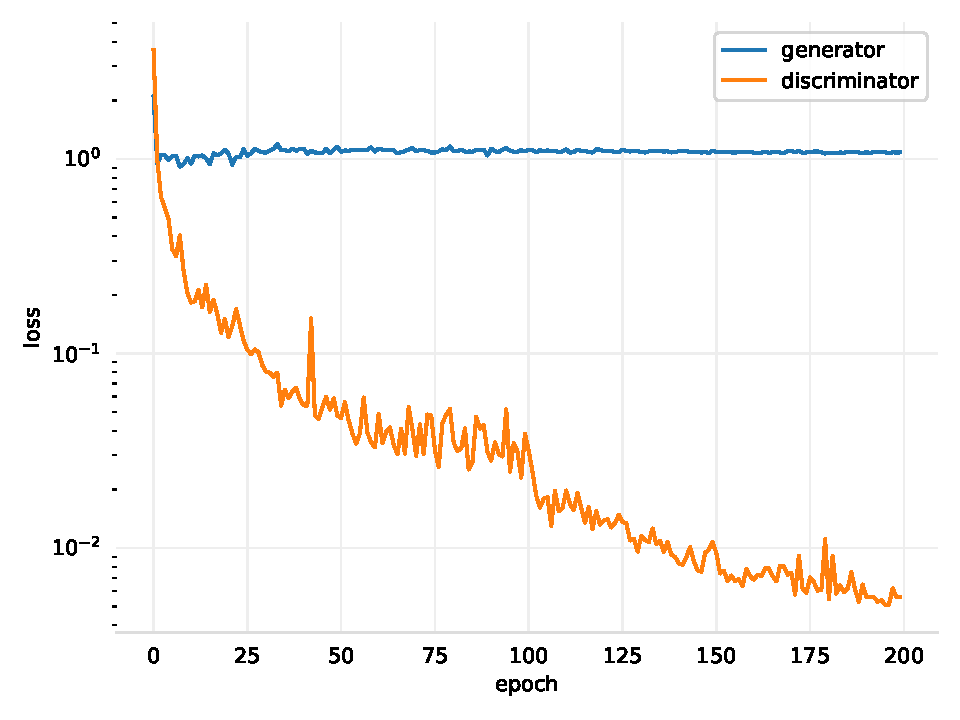
\includegraphics[width=\textwidth]{resources/png/gan-losses/batch-limited.pdf}
            \caption{Losses for the limitation of batches.}
        \end{subfigure}
        \hfill
        \begin{subfigure}[b]{0.22\textwidth}
            \centering
            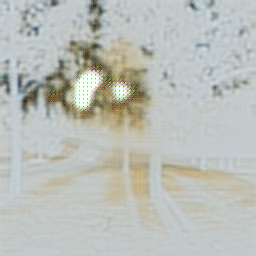
\includegraphics[width=\textwidth]{resources/png/gan-results/batch-limitation.png}
            \caption{Result obtained.}
            \label{fig:limitation}
        \end{subfigure}
        \caption{Results obtained for the limitation of number of batches per epoch.}
    \end{figure}
    
    \subsubsection{Training only one model}
    
    Since we are not interested to go from painting to photograph for this task, we have tried to only train one generator and one discriminator (thus removing the term cycle in CycleGAN) on the testing set (120 images of Monet and 750 images of landscapes). The results were quite promising, but we realized that all input images output close images to one another. We believe this is due to the fact that we only had for the generator loss the adversarial one, and so our model may well have overfitted or gone into mode collapse (since all its predictions went to close outputs). To try to solve that, we have launched the same experiment, but implemented the identity loss described by the authors (the loss compares the result of the passage of an image from the Monet painting in the painting-to-landscape generator to the same image, since the network should then output an image that is ideally identical to the input one). We believed that should solve the fact that all input images lead to close outputs. The loss and result obtained for this idea without the identity loss is given at Figure \ref{fig:one1}. As can be seen, the two losses evolve in opposite fashion and, at one point, the generator loss decreased vastly while the discriminator one increased. Decreasing the learning rate at that point might have been a good idea, however we had no idea about the behaviour to expect from this test and used the learning rate of the original architecture and did not save intermediate models.
    
    \begin{figure}[H]
        \centering
        \begin{subfigure}[b]{0.22\textwidth}
            \centering
            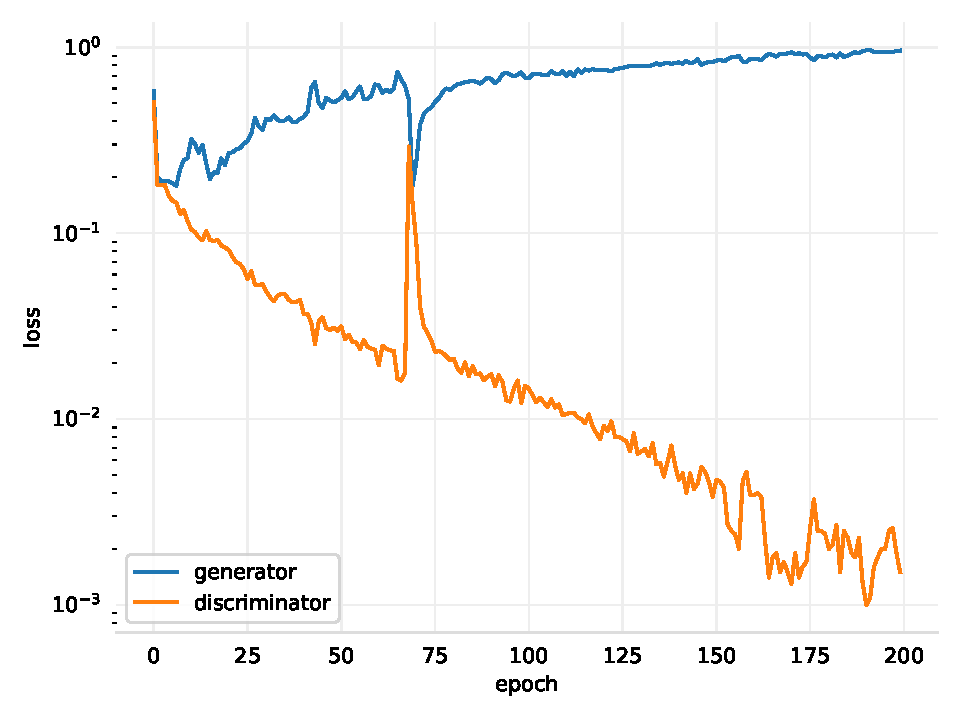
\includegraphics[width=\textwidth]{resources/png/gan-losses/one1.pdf}
            \caption{Losses for only one model.}
        \end{subfigure}
        \hfill
        \begin{subfigure}[b]{0.22\textwidth}
            \centering
            \includegraphics[width=\textwidth]{resources/png/gan-results/test_one.png}
            \caption{Result obtained.}
            \label{fig:one1}
        \end{subfigure}
        \caption{Results obtained for training only one generator and discriminator.}
    \end{figure}
    
    The results for the models to which we added the identity loss are given at Figure \ref{fig:one2}. The model also includes a LR scheduler that reduces the learning rate when it detects a plateau for both generator and discriminator (although it may have been better to only use it on the generator). The initial scheduler provided worse results, all other things being equal, than the plateau one. As can be seen, the loss for the generator first decreases before increasing. This does not mean that the output images get worse but rather that the discriminator becomes too good, since the results are not that bad. They indeed resemble the input images and have a painting feel, although we had to reduce the training dataset size and the number of epochs to get results before the deadline, so letting it train longer may well yield better results (we will let it run longer to get results for the presentation). Although the generator loss end up increasing, the results are better than for the previous tests.
    
    \begin{figure}[H]
        \centering
        \begin{subfigure}[b]{0.22\textwidth}
            \centering
            \includegraphics[width=\textwidth]{resources/png/gan-losses/onemodid.pdf}
            \caption{Losses.}
        \end{subfigure}
        \hfill
        \begin{subfigure}[b]{0.22\textwidth}
            \centering
            \includegraphics[width=\textwidth]{resources/png/gan-results/onemodid.png}
            \caption{Result obtained.}
            \label{fig:one2}
        \end{subfigure}
        \caption{Results obtained for training only one generator and discriminator, using a LR scheduler and the identity loss.}
    \end{figure}
    
    \subsubsection{Training on less data}
    
    Instead of limiting the number of batches but keeping the whole training dataset, as we did for the first strategy described here, we decided to restrict ourselves to a smaller dataset, but each epoch would see each sample through. The datasets chosen were simply the pruned training ones (50 Monet painting and 120 landscapes), and the results are given at Figure \ref{fig:less1}. The loss behaves as for the limitation of the number of epochs, and the result is simply a paler version of the input. Maybe, this time, the dataset was not exhaustive enough for the model to pick up Monet's style.
    
    \begin{figure}[ht]
        \centering
        \begin{subfigure}[b]{0.22\textwidth}
            \centering
            \includegraphics[width=\textwidth]{resources/png/gan-losses/testless.pdf}
            \caption{Losses for the training on less data.}
        \end{subfigure}
        \hfill
        \begin{subfigure}[b]{0.22\textwidth}
            \centering
            \includegraphics[width=\textwidth]{resources/png/gan-results/less1.png.png}
            \caption{Result obtained.}
            \label{fig:less1}
        \end{subfigure}
        \caption{Results obtained for the limitation on the training dataset size.}
    \end{figure}
    
    Other tests have been made without success and are not reported here, and more results are given in the appendix \ref{add} and not here because the models did not have the time to run to completion due to a high utilization of the GPU cluster for the last week of the semester, and because our models take tens of hours to train (and thus we are only able to build on top of our discoveries after the training is complete, which was delayed since we were not prioritized due to the high training time required). Better results should however be obtained when these models have completed their training.
    
    
    %%%%%%%%%%%%%%%%%%%%
    %%%%%%%%%%%%%%%%%%%%
    %%%%%%%%%%%%%%%%%%%%
    
    % ----- Discussion ----- %
    
    % TO DO
    % -----
    % A critical discussion of the performance of the neural network, analysis of the potential limitations, tips for future work
    
    \section{Discussion}\label{sec:discussion}
    
    \subsection{Neural style transfer (Gatys et al.)}
    
    Our implementation of the technique of Gatys et al. is quite faithful to the original paper. Although inspired by tutorials, we have added our own personal touch in order to re-implement certain aspects and to better understand it.\\
    
    The results we get seem good at first glance. However, the field of style transfer is very rich and has evolved a lot since the publication of the paper by Gatys et al. \cite{DBLP:journals/corr/GatysEB15a} and many methods that drastically improve the results have emerged. We have focused here on the basic principles but a whole range of improvements could have been possible. Our model has its limitations in that, given the rapidly stabilizing loss functions, we cannot get much better results just by playing with the basic parameters, although our results are very good in our opinion.\\
    
    We used a pre-trained model for this project. We didn't bother trying to train the model by ourselves as it would have been very time consuming and not really related to our topic. However, training a model (e.g. VGG19) with a wide range of artistic images (paintings, etc.) might have led, maybe, to better results (although we believe that not using a model pretrained on object recognition would have actually lead to worse results).\\
    
    Finally, we realized how much deep learning techniques, even modern ones, require a lot of work on parameters and training in order to obtain suitable results. Moreover, a series of parameters that give suitable results for one image will not give suitable results for another; it is difficult to generalize the model.\\
    
    We are satisfied with the results we are achieving. It is difficult to judge their quality from a quantitative point of view since this is a very subjective application, but nevertheless, from a qualitative point of view, the results are very appealing.
    
    \subsection{CycleGAN (Zhu et al.)}
    
    The results obtained from CycleGAN were very disappointing at first, and we had to try numerous changes to finally obtain something that produced results that were not completely horrid. The best results were obtained from training a single GAN model (one generator and one discriminator), while CycleGAN provided bad results, probably because we did not provide a big enough dataset due to time restrictions (training on the original dataset would have taken weeks). For our application, since we did not need to go from painting to landscape, a simple GAN network might have been better (at least easier to train) but a CycleGAN has proved to provide good results nonetheless in the authors' paper and experiments. The use of a plateau learning rate scheduler improved somewhat the results, compared with the technique of the authors. The main limitation is that, in this state, this CycleGAN implementation does not provide acceptable results. The improved solutions that are being trained are discussed in the appendix C and will be showed at the presentation if they prove successful. One other big limitation of this method is the time needed to train the network and the impossibility to generalize its results, as will be discussed in the section below.\\
    
    After comparing our implementation with that of the author and other found on the internet, and asking an assistant, we believe that our implementation is not wrong, and so the only thing we did differently from the authors was not train on the whole training dataset (which was not possible in our case). If our other tests do not yield good results, this will be our hypothesis for our disappointing results. During this project, we learned that training a GAN network was not an easy task, since two networks were working to achieve two opposite goals. We expected to get better results more easily.
    
    \subsection{Comparison between the two solutions}
    
    As can be understood from the papers, CycleGAN is a general tool used to go from domain to domain, whatever these domains. It has therefore not been tailored with neural style transfer in mind, but works quite well on that task, although the training time and resources required to obtain satisfactory results are much more expensive than for the other paper. Indeed, CycleGAN requires a dataset of images from both domains to be able to train, and the greater the size of those datasets, the better the results, whereas the solution proposed by \cite{DBLP:journals/corr/GatysEB15a} needs only the content image and the style image. It is therefore much more flexible than CycleGAN because it can take almost any content and style images and provide good results immediately (with some tweaking of parameters maybe required), while CycleGAN is trained on two specific domains. In our implementation we chose Monet paintings and landscapes, and the model trained on those, which means that it will not be able to translate input images in another style than Monet without training it on that particular style, and that is something that is not necessarily possible for generic styles (a painter has a style that it uses in hundreds of paintings, whereas a random image may be one of a kind, leading to an impossible translation by CycleGAN).\\
    
    With that being said, CycleGAN provides better, more natural results than the other solution for two given domains, because it learns the style of the painter (or the artist) instead of the style of a given painting or art piece, but at the cost of a training process involving thousands of images and hundreds of hours, which make it less versatile than Gatys' solution, which works on the fly.
    
    
    %%%%%%%%%%%%%%%%%%%%
    %%%%%%%%%%%%%%%%%%%%
    %%%%%%%%%%%%%%%%%%%%
    
    % ----- APPENDIX ----- %
    
    \appendix
    
    %%%%%%%%%%%%%%%%%%%%
    %%%%%%%%%%%%%%%%%%%%
    %%%%%%%%%%%%%%%%%%%%
    
    % ----- Deep learning terms used ----- %
    
    \section{Deep Learning terms used}
    
    Since we were asked to describe what we did as if the reader had never taken a Deep Learning course, we gather here the different concepts used in this report, and give them personal definitions (helped at times with the slides of Introduction to Machine Learning given by Mr Geurts and Wehenkel during the first semester) :
    
    \begin{itemize}
        \item \textbf{Convolutional layer} : A convolutional layer simply applies a filter to its input. That filter is a matrix, which computes, for each element of the input (representing usually a pixel), a weighted sum of its neighbours. This allows to detect local features. The output of such a filter is thus called a \textbf{feature map}.
        
        \item \textbf{Pooling layers} : A pooling layer (or subsampling layer) is used to aggregate values in a local region, thus reducing the size of the output compared to the input. The two types of pooling layers used in our implementations were the average pooling (the aggregated value is the average of the region) and the max pooling (the aggregated value is the local maximum of the region).
        
        \item \textbf{Loss} : A loss is the function that is used in order to evaluate the candidate solutions (set of weights of the network, network architecture,...) to the tasks. The optimal solution maximizes (or minimizes) such a loss and is approximated through (or found by, depending on the algorithm) optimization algorithms. Such a function helps describing the goodness of a complex structure with a single number\cite{loss}.
        
        \item \textbf{Fully-connected layer} : Such layers are usually used to combine the features previously extracted by convolutional layers in a non-linear way. Indeed, these layers act as universal function approximators (when there are at least two of them).
        
        \item \textbf{Normalization layer} : Such a layer is used to normalize the input via a mean and a standard deviation. Those two values used in our network have been empirically derived by the authors of VGG.
        
        \item \textbf{ReLU} : A rectifier linear unit is an activation function that is zero for all negative inputs and the value of the input otherwise. An activation layer is used to transform the output of a layer and add it non-linearities.
        
        \item \textbf{GAN} : This term has already been extensively defined when talking about CycleGAN.
        
        \item \textbf{Backpropagation} : This algorithm is used to adjust the different parameters of a network in order to decrease the loss (or increase it if we want a high loss).
        
        \item \textbf{Learning rate} : The learning rate is the step size at each iteration of the optimization algorithm (gradient descent). A high rate will allow high steps in the loss plane while a smaller rate will force the loss to move in its near neighbourhood. For such a reason, we usually set a high rate at the beginning and decrease it over time, so that the algorithm can converge to a local minimum and not jump out of the potential well (if the learning rate is too large, the loss may inevitably exit the well).
    \end{itemize}
    
    %%%%%%%%%%%%%%%%%%%%
    %%%%%%%%%%%%%%%%%%%%
    %%%%%%%%%%%%%%%%%%%%
    
    % ----- CycleGAN additional results ----- %
    
    \section{CycleGAN additional results}\label{add}
    
    This appendix contains further tests of different parameters of CycleGAN.
    
    \subsection{Dataset size}
    
    Although it could not be tested thoroughly, we believe that, for a given model, the bigger the training set the better the results. The results given in Figure \ref{fig:trainingsizes}. They were tested for 60 epochs, since we had a time limit, and the results are shown on one of the training images. As can be seen, the larger dataset yields better results, although, for a size of 120+750 images, we get worse performances, probably because the number of epochs should be made bigger for larger datasets, and because the loss suddenly increased in the training, since we used the learning rate of the authors. No conclusion can thus be made, but our belief is that larger training datasets yield better results and better generalisation. Models should have been trained on 200 epochs, as the authors do, but the utilization of the GPUs during the last week was too high for these models to finish. The results of this ongoing experiment will be displayed at the presentation.
    
    \begin{figure}[ht!]
        \centering
        \begin{subfigure}[b]{0.22\textwidth}
            \centering
            \includegraphics[width=\textwidth]{resources/png/gan-results/inc1030.png}
            \caption{Dataset of 10+30 images.}
        \end{subfigure}
        \hfill
        \begin{subfigure}[b]{0.22\textwidth}
            \centering
            \includegraphics[width=\textwidth]{resources/png/gan-results/inc50150.png}
            \caption{Dataset of 50+150 images.}
            \label{fig:trainingsizes}
        \end{subfigure}
        \caption{Training dataset sizes results.}
    \end{figure}
    
    \subsection{Other ongoing experiments}
    
    Some of the models that are still training are :
    \begin{itemize}
        \item The adding of the identity loss to the general model.
        \item The same as above, but with a smaller dataset.
        \item The training of the general model with some tensors detached at different places to try to get the generators to perform better, with and without the identity loss.
        \item The same as above, but with a plateau LR scheduler.
    \end{itemize}
    
    Although they were launched on a Monday, these models had to wait until Thursday to be launched on the cluster, and thus have not completed the training as of Friday (and training without a GPU was not possible). However, should the results be satisfactory, which we believe they will, since these changes build upon previous successful discoveries, they will be showcased on the day of the presentation.
    
    \section{CycleGAN full architecture}
    
    These architectures are taken verbatim from the authors' paper.\\
    
    For the \textbf{generator} : \\
    
    Let c7s1-k denote a 7x7 Convolution-InstanceNormReLU layer with k filters and stride 1. dk denotes a 3 x 3 Convolution-InstanceNorm-ReLU layer with k filters and stride 2. Reflection padding was used to reduce artifacts. Rk denotes a residual block that contains two 3 x 3 convolutional layers with the same number of filters on both layer. uk denotes a 3 x 3 fractional-strided-ConvolutionInstanceNorm-ReLU layer with k filters and stride $\frac{1}{2}$.\\
    
    The network with 6 residual blocks consists of :\\
    
    c7s1-64,d128,d256,R256,R256,R256,R256,R256,
    R256,u128,u64,c7s1-3\\
    
    The network with 9 residual blocks consists of :\\
    
    c7s1-64,d128,d256,R256,R256,R256,
    R256,R256,R256,R256,R256,R256,u128,u64,c7s1-3\\
    
    For the \textbf{discriminator}:\\
    
    Let Ck denote a 4 x 4 Convolution-InstanceNorm-LeakyReLU layer with k filters and stride 2. After the last layer, we apply a convolution to produce a 1-dimensional output. We do not use InstanceNorm for the first C64 layer. We use leaky ReLUs with a slope of 0.2.\\
    
    The discriminator architecture is :\\
    
    C64-C128-C256-C512\\
    
    However, in their implementation, the authors added after C512 another block containing a Conv layer outputing 512 channels, followed by an InstanceNorm and a LeakyReLU, before the final convolutional layer.
    
    %%%%%%%%%%%%%%%%%%%%
    %%%%%%%%%%%%%%%%%%%%
    %%%%%%%%%%%%%%%%%%%%
    
    % ----- References ----- %
    
    \newpage
    
    \bibliographystyle{unsrt}
    \bibliography{references.bib}
    \nocite{*}
\end{document}
